
\question[6] (6分)某同学利用图(a)所示装置验证动能定理。调整木板的倾角平衡摩擦阻力后,挂上钩码,钩码下落,带动小车运动并打出纸带。某次实验得到的纸带及相关数据如图(b)所示。\begin{center}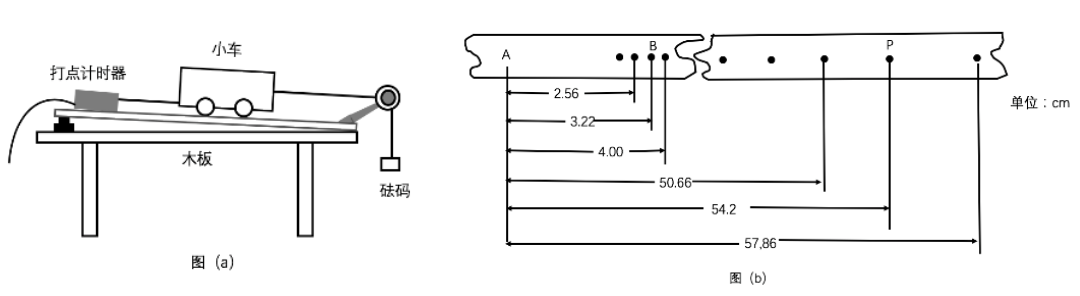
\includegraphics[width=14cm]{img/image7.png}\end{center}已知打出图(b)中相邻两点的时间间隔为$0.02s$,从图(b)给出的数据中可以得到,打出B点时小车的速度大小$v_B=$\key{0.36}$m/s﹐$打出Р点时小车的速度大小$v_P=$\key{1.80}$m/s$。(结果均保留2位小数)若要验证动能定理,除了需测量钩码的质量和小车的质量外,还需要从图(b)给出的数据中求得的物理量为\key{B、P 之间的距离}.
\question[6] (9分)已知一热敏电阻当温度从$10°C$升至$60°C$时阻值从几千欧姆降至几百欧姆,某同学利用伏安法测量其阻值随温度的变化关系.所用器材:电源E、开关S、滑动变阻器R(最大阻值为$20Ω$)、电压表(可视为理想电表)和毫安表(内阻约为$100Ω$).

(1)在答题卡上所给的器材符号之间画出连线,组成测量电路图\begin{center}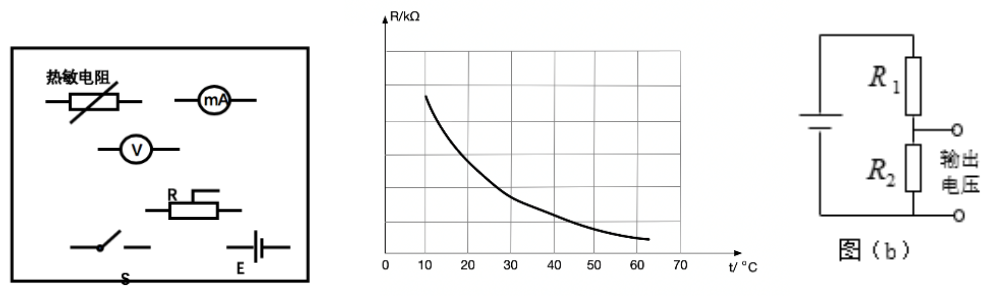
\includegraphics[width=14cm]{img/image8.png}\end{center}

(2)实验时,将热敏电阻置于温度控制室中,记录不同温度下电压表和毫安表的示数,计算出相应的热敏电阳阻值。若某次测量中电压表和毫安表的示数分别为$5.5V$和$3.0mA$,则此时热敏电阻的阻值为\key{1.8}(保留2位有效数字)。实验中得到的该热敏电阻阻值R随温度t变化的曲线如图(a)所示

(3)将热敏电阻从温控室取出置于室温下,测得达到热平衡后热敏电阻的阻值为$2.2kΩ$。由图(a)求得,此时室温为\key{25.5}◦C保留3位有效数字)。

(4)利用实验中的热敏电阻可以制作温控报警器,其电路的一部分如图(b)所示。图中,E为直流电源(电动势为$10V$,内阻可忽略);当图中的输出电压达到或超过$6.0V$时,便触发报警器(图中未画出)报警。若要求开始报警时环境温度为$50°C$,则图中\key{$R_1$}(填$"R_1"$或$"R_2"$)应使用热敏电阻,另一固定电阻的阻值应为\key{1.2}kΩ(保留2位有效数字)。

\newpage
\question[6] (12分)如图,一边长为$l_0$的正方形金属框$abcd$固定在水平面内,空间存在方向垂直于水平面、磁感应强度大小为B的匀强磁场。一长度大于$\sqrt{2}l_{0}$的均匀导体棒以速率v自左向右在金属框上匀速滑过,滑动过程中导体棒始终与ac垂直且中点位于ac上,导体棒与金属框接触良好。已知导体棒单位长度的电阻为r,金属框电阻可忽略。将导体棒与a点之间的距离记为x,求导体棒所受安培力的大小随x($0\leqslant x\leqslant \sqrt{2}l_{0}$)变化的关系式。\begin{center}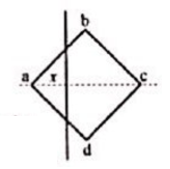
\includegraphics[]{img/image9.png}\end{center}
\begin{solution}{4cm}
当导体棒与金属框接触的两点间棒的长度为 时,由法拉第电磁感应定律知,导体棒上感应电动势的大小为

E=Blv\ding{172}

由欧姆定律,流过导体棒的感应电流为

$I= \frac{E}{R}$ \ding{173}

式中, 为这一段导体棒的电阻,按题意有

$R = rl$\ding{174}

此时导体棒所受安培力大小为

$f = BlI$\ding{175}

由题设和几何关系有
$l= 
\begin{cases} 
    2x,0 \leqslant x \leqslant \frac{ \sqrt{2}}{2}l_{0}\\\\ 
    2( \sqrt{2}l_{0}-x), \frac{ \sqrt{2}}{2}I_{0}<x \leqslant \sqrt{2}l
\end{cases}     $   \ding{176}

联立\ding{172}\ding{173}\ding{174}\ding{175}\ding{176}式得

$f=
\begin{cases}
    \frac{2B^{2}v}{r}x,0 \leqslant x \leqslant \frac{ \sqrt{2}}{2}l_{0}\\\\
    \frac{2B^{2}v}{r}( \sqrt{2}l_{0}-x),\frac{ \sqrt{2}}{2}l_{0}<x \leqslant \sqrt{2}l_0
\end{cases}
$ 
\end{solution}

\newpage
\question[6] (20分)如图,相距$L=11.5m$的两平台位于同一水平面内,二者之间用传送带相接。传送带向右匀速运动,其速度的大小v可以由驱动系统根据需要设定。质量$m=10kg$的载物箱(可视为质点),以初速度$v_0=5.0m/s$自左侧平台滑上传送带。载物箱与传送带间的动摩擦因数$μ=0.10$,重力加速度取$g=10m/s^2$。

(1)若$v=4.0m/s$,求载物箱通过传送带所需的时间;

(2)求载物箱到达右侧平台时所能达到的最大速度和最小速度;

(3)若$v=6.0m/s$,载物箱滑上传送带$\Delta t=\frac{13}{12}s$后,传送带速度突然变为零.求载物箱从左侧平台向右侧平台运动的过程中,传送带对它的冲量.\begin{center}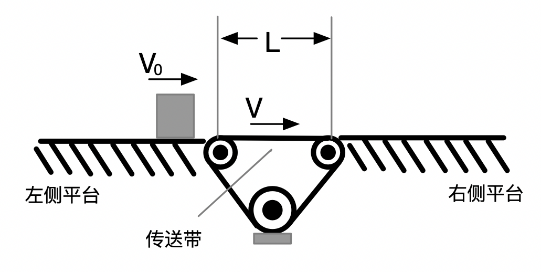
\includegraphics[]{img/image10.png}\end{center}
\begin{solution}{4cm}
(1)
$μ mg = ma$

$t  = \frac{V_{0}-V}{a}=1s$

$x_{1}= \frac{V_{0}+V}{2} \cdot t_{1}=4.5m$

$x_{2}=L-x_{1}= \nu \cdot t_{2}$

$t=t_{1}+t_{2}=2.75s$

(2)
$v_{ \max }^{2}-v_{0}^{2}=2aL$

$v_{ \max }=4 \sqrt{3}m/s$

$v _{0}^{2}- \nu _{ \min }^{2}=2aL$

$v_{\min}= \sqrt{2}m/s$   

(3)
$x_{3}= \frac{v+v_{0}}{2}t_{3}=5.5m$

$t_{4}= \Delta t-t_{3}= \frac{1}{12}s$

$x _4 = v · t _4 = 0 . 5 m$

$x _5 = L - x _4- x _5 = 5 . 5 m$

$v ^2- v _t^ 2 = 2 ax _5$

$v_t = 5 m / s$, 减速时间和加速时间相同

$I _f = mv_t - mv _0 = 0$

$I_\text{带} = I _N +1 _f = I _N$

$I_{N}=I_{G}=mg( \Delta t+t_{2})= \frac{625}{3}N \cdot S$

方向垂直向上  
\end{solution}

\newpage
\question[6] [物理——选修$3–3$](15分)

(1)(5分)如图,一开口向上的导热气缸内。用活塞封闭了一定质量的理想气体,活塞与气缸壁间无摩擦。现用外力作用在活塞上。使其缓慢下降。环境温度保持不变,系统始终处于平衡状态。在活塞下降过程中\key{BCD}。(填正确答案标号。选对1个得2分。选对2个得4分,选对3个得5分;每选错1个扣3分,最低得分为0分)\begin{center}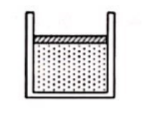
\includegraphics[]{img/image11.png}\end{center}
A.气体体积逐渐减小,内能增知

B.气体压强逐渐增大,内能不变

C.气体压强逐渐增大,放出热量

D.外界对气体做功,气体内能不变

E.外界对气体做功,气体吸收热量

(2)(10分)如图,两侧粗细均匀、横截面积相等、高度均为$H=18cm$的U型管,左管上端封闭,右管上端开口.右管中有高$h_0=4cm$的水银柱,水银柱上表面离管口的距离$1=12cm.$管底水平段的体积可忽略.环境温度为$T_1=283K.$大气压强$P_0=76cmHg.$(i)现从右侧端口缓慢注入水银(与原水银柱之间无气隙),恰好使水银柱下端到达右管底部.此时水银柱的高度为多少?(ii)再将左管中密封气体缓慢加热,使水银柱上表面恰与右管口平齐,此时密封气体的温度为多少?\begin{center}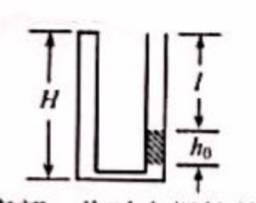
\includegraphics[]{img/image12.png}\end{center}
\begin{solution}{4cm}
(i)
设密封气体初始体积为 $V _1$ , 压强为 $p _1$ , 横截面积为 S , 密封气体先经等温压缩过程体积变为$ V _2$ , 压强变为 $p _2$ . 由玻意耳定律有
$p _1V _1 = p _2 V _2$ \ding{172} 

设注入水银后水银柱高度为 h , 水银的密度为 ρ , 按题设条件有

$p _1 = p _0+ ρ gh _o$ \ding{173} 
$p _2 = p _0+ ρ gh$ \ding{174} 
$V _1 = ( 2 H - l - h ) S$ , $V _2 = HS$ \ding{175} 

联立\ding{172}\ding{173}\ding{174}\ding{175}式并代入题给数据得

$h = 12 . 9 cm$ \ding{176}

(ii)
密封气体再经等压膨胀过程体积变为 $V _1 $, 温度变为 $T _1$ , 由盖 - 吕萨克定律有
$\frac{V_{2}}{T_{1}}= \frac{V_{3}}{T_{2}}$\ding{177}

按题设条件有 $V _3 = ( 2 H - h ) S$ \ding{178} 

联立\ding{175}\ding{176}\ding{177}\ding{178}式并代入题给数据得 $T _2 = 363 K$   
\end{solution}
\newpage
\question[6] [物理选修$3–4$](15分)

(1)(5分)如图,一列简谐横波平行于x轴传播,图中的实线和虚线分别为$t=0$和$t=0.1s$时的波形图。已知平衡位置在$x=6m$处的质点,在0到$0.1s$时间内运动方向不变。这列简谐波的周期为\key{0.4s}s,波速为\key{10m/s}$m/s$,传播方向沿x轴\key{负方向}(填“正方向”或“负方向”)。\begin{center}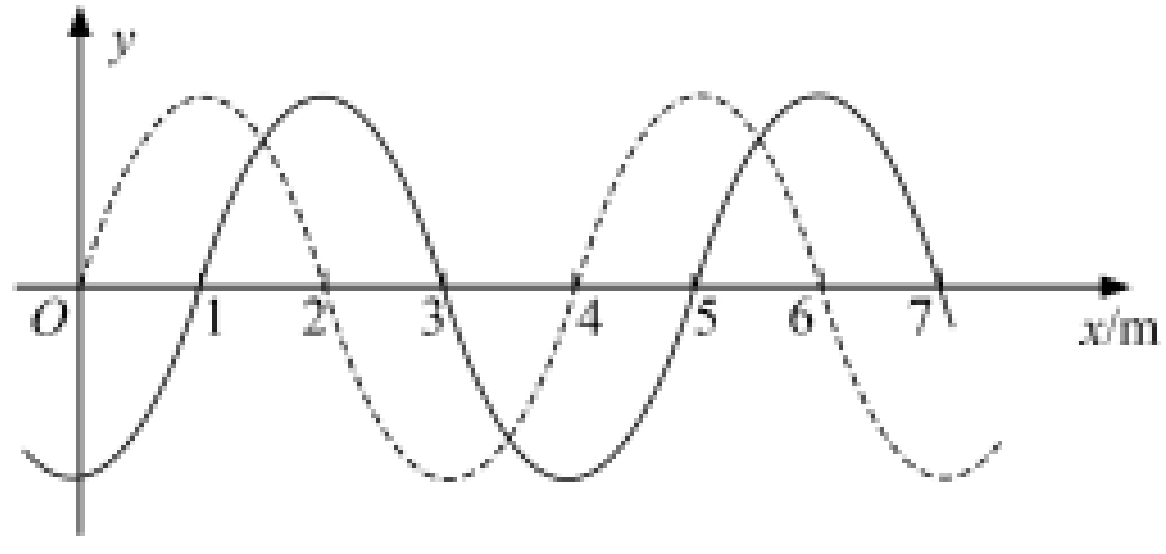
\includegraphics[width=4cm]{img/image13.png}\end{center}

(2)(10分)如图,一折射率为的材料制作的三棱镜,其横截面为直角三角形$ABC$,$\angle A=90^∘$,$\angle B=30^∘$。一束平行光平行于BC边从AB边射入棱镜,不计光线在棱镜内的多次反射,求AC边与BC边上有光出射区域的长度的比值。\begin{center}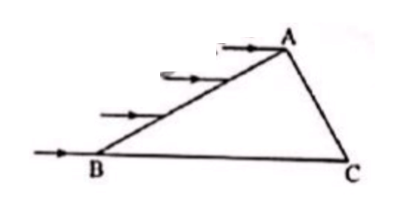
\includegraphics[]{img/image14.png}\end{center}
\begin{solution}{4cm}
如图 ( a ) 所示 , 设从 D 点入射的光线经折射后恰好射向 C 点 , 光在 AB 边上的入射角为 $θ 1$ , 
折射角为 $θ_2$ , 由折射定律有 $sin θ , = nsin θ _2$ \ding{172} 
\begin{center}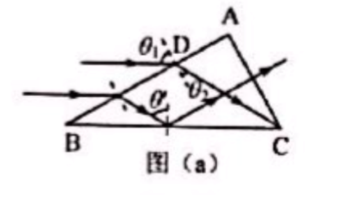
\includegraphics[]{img/image15.png}\end{center}
设从 DB 范围入射的光折射后在 BC 边上的入射角为 $θ ^\prime$ , 由几何关系 $θ ^\prime = 30 ^∘ + θ _2$ \ding{173}小由\ding{172}\ding{173}式并代入题给数据得
$θ_2  = 30 °$\ding{174}
$nsin θ > 1$ \ding{175} 

所以 , 从 DB 范围入射的光折射后在 BC 边上发生全反射 , 反射光线垂直射到 AC 边 ,AC边上全部有光射出 .

设从 AD 范围入射的光折射后在 AC 边上的入射角为 $θ ^\prime$ , 如图 ( b ) 所示 . 由几何关系

$θ ^\prime = 90 ° - θ _2$ \ding{176} 
\begin{center}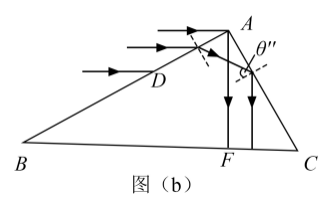
\includegraphics[width=4cm]{img/image16.png}\end{center}
由\ding{174}\ding{176}式和已知条件可知 
$nsin θ > 1$ \ding{177} 

即从 AD 范围入射的光折射后在 AC 边上发生全反射 , 反射光线垂直射到 BC 边上 .设 BC 边上有光线射出的部分为 CF , 由几何关系得 
$CF = AC · sin 30 ^∘$\ding{178} 

AC边与 BC 边有光出射区域的长度的比值为 

$\frac{AC}{CF}=2$ \ding{179} 
\end{solution}
